% !TEX program = xelatex
% A0 portrait: 841 x 1189 mm. Print at 100% / actual size.
\RequirePackage{fix-cm}
\documentclass{article}
\usepackage[paperwidth=84.1cm,paperheight=118.9cm,margin=0cm]{geometry}
\usepackage{lmodern}
\usepackage{fontspec,graphicx,xcolor,tikz,amsmath,booktabs,qrcode,hyperref}
\setsansfont{texgyreheros}[WordSpace=1.2,Extension=.otf,UprightFont=*-regular,BoldFont=*-bold,ItalicFont=*-italic,BoldItalicFont=*-bolditalic]
\renewcommand{\familydefault}{\sfdefault}
\usetikzlibrary{arrows.meta,positioning,calc}
% Canonical author and credit strings copied from the checked paper.
\newcommand{\PaperTitle}{Fossil Fuel Prices and Capital Cost: A Machine Learning Driven Study on Energy Transition}
\newcommand{\AuthorNames}{Shilin Ou, Luyao Zhang, and Ming-Chun Huang}
\newcommand{\AuthorNamesMarked}{Shilin Ou\textsuperscript{\dag}, Luyao Zhang\textsuperscript{*}, and Ming-Chun Huang\textsuperscript{*}}
\newcommand{\PaperAffiliation}{Duke Kunshan University, Suzhou, China}
\newcommand{\PresenterName}{Shilin Ou}
\newcommand{\PresenterEmail}{shilin.ou@dukekunshan.edu.cn}
\newcommand{\CorrespondenceText}{Corresponding authors: Zhang: luyao.zhang@dukekunshan.edu.cn, Social Science Division and Digital Innovation Research Center; Huang: mingchun.huang@dukekunshan.edu.cn, Natural and Applied Science Division and Digital Innovation Research Center, Duke Kunshan University. Address: No.8 Duke Ave., Kunshan, Jiangsu 215316, China.}
\newcommand{\FundingText}{The Duke Kunshan University Education Development Foundation supports the research. The research results of this article are also sponsored by the Kunshan Municipal Government research funding.}
\newcommand{\AuthorNoteText}{Shilin benefited from scholarly exchange with participants in the AAAI-26 Workshop on AI for Environmental Science, held on January 27, 2026, at the Singapore EXPO in Singapore. Shilin gratefully acknowledges the Travel Grant provided by the Duke Kunshan University Office of Academic Services, which supported participation in the workshop.}
\newcommand{\PreparationText}{OpenAI Codex assisted language and consistency revisions throughout the manuscript, preparation of Fig. 1, and correction of the sensitivity-analysis code.}
\newcommand{\CodeURL}{https://github.com/GreenComp-ERC/ImpactOfFossilFeulPrice}
\newcommand{\DataURL}{https://huggingface.co/datasets/global-nomad-nexus/ImpactOfFossilFuelPrice-WACC}
\newcommand{\EventName}{2026 Asian Conference on Artificial Intelligence Technology}
\newcommand{\EventShort}{ACAIT 2026}
\newcommand{\EventPlace}{Chongqing, China}

\definecolor{Navy}{HTML}{012169}
\definecolor{Blue}{HTML}{00539B}
\definecolor{Teal}{HTML}{247F83}
\definecolor{Gold}{HTML}{B3853A}
\definecolor{Muted}{HTML}{4E5A66}
\definecolor{Pale}{HTML}{EEF5FA}
\pagestyle{empty}
\setlength{\parindent}{0pt}
\hypersetup{pdftitle={\PaperTitle: A0 poster},pdfauthor={Shilin Ou, Luyao Zhang, Ming-Chun Huang},colorlinks=true,urlcolor=Blue}
\graphicspath{{../shared/figures/}}
\newcommand{\posthead}[2]{{\fontsize{19}{23}\selectfont\color{Teal}#1}\quad{\fontsize{35}{42}\selectfont\bfseries\color{Navy}#2}\par\vspace{0.55cm}}
\newcommand{\bodyfont}{\fontsize{25}{33}\selectfont\color{black!85}}
\newcommand{\captionfont}{\fontsize{21}{27}\selectfont\color{Muted}}
\newcommand{\footfont}{\fontsize{18}{23}\selectfont\color{black!80}}
\begin{document}
\null
\begin{tikzpicture}[remember picture,overlay,x=1cm,y=-1cm]
\coordinate (O) at (current page.north west);
\begin{scope}[shift={(O)}]
\fill[white] (0,0) rectangle (84.1,118.9);
\node[anchor=north west,inner sep=0] at (3,2) {
\includegraphics[width=10.0cm]{acait_logo.png}};
\node[anchor=north east,inner sep=0] at (81.1,2.2) {
\includegraphics[width=16.0cm]{dku_logo.png}};
\node[anchor=north west,inner sep=0,text width=63cm,font=\fontsize{21}{26}\selectfont,text=Muted] at (16,2.6) {\EventName\\\EventPlace\quad|\quad AI for Better Life};

\node[anchor=north west,inner sep=0,text width=78.1cm,text=Navy] at (3,7.4) {\fontsize{65}{74}\selectfont\bfseries Fossil Fuel Prices and Capital Cost:\\A Machine Learning Driven Study\\on Energy Transition};
\node[anchor=north west,inner sep=0,text width=78.1cm] at (3,16.0) {\fontsize{30}{38}\selectfont\AuthorNamesMarked\\[0.25cm]\fontsize{25}{32}\selectfont\PaperAffiliation};
\draw[Teal,line width=2.2pt] (3,20.2)--(81.1,20.2);

\fill[Pale] (3,21.4) rectangle (81.1,27.0);
\node[anchor=north west,inner sep=0,text width=74cm] at (5.1,22.4) {\fontsize{31}{40}\selectfont\bfseries\color{Navy}An AI workflow connects energy-price signals with financing scenarios.\\[0.35cm]\bodyfont Regional fit differs, wind and solar fit most closely, and time-split checks show where price signals add information beyond a trend.};

% LEFT COLUMN
\node[anchor=north west,inner sep=0,text width=37cm] at (3,29.5) {
\posthead{01}{Question and data}
\bodyfont How do fossil fuel prices and inflation relate to energy-project WACC across China, Europe, and the Middle East?\\[0.5cm]
\textbf{3 regions}\quad\textbf{9 technologies}\quad\textbf{120 monthly rows}\\[0.35cm]
Historical price and macroeconomic inputs are paired with 2026--2035 WACC projections from Calcaterra et al. (2024). Coal and gas generation are conventional-technology comparisons.
};

\node[anchor=north west,inner sep=0,text width=37cm] at (3,41.6) {\posthead{02}{Three-stage framework}};
\begin{scope}[shift={(3,45.0)},font=\fontsize{24}{31}\selectfont,>=Latex,
 stage/.style={anchor=north west,draw=black!20,rounded corners=2pt,text width=32.5cm,minimum height=5.1cm,inner sep=0.65cm,align=left}]
\node[stage,fill=Pale] (s1) at (0,0) {\textbf{1\quad Fuel-price forecasts}\\CNN, LSTM/GRU, attention, and Gaussian-process smoothing};
\node[stage,fill=Teal!6] (s2) at (0,7.0) {\textbf{2\quad Regional inflation}\\LSTM + feed-forward network; five-model ensemble};
\node[stage,fill=Gold!7] (s3) at (0,14.0) {\textbf{3\quad WACC comparisons}\\AutoGluon regressions by region, fuel, and technology};
\draw[->,Teal,line width=2.2pt] (s1.east)--++(1.1,0)|-(s3.east);
\draw[->,Teal,line width=2.2pt] ($(s2.south)+(0,0.15)$)--($(s3.north)+(0,-0.15)$);
\end{scope}

\node[anchor=north west,inner sep=0,text width=37cm] at (3,66.6) {\posthead{03}{Archived price comparison}};
\node[anchor=north west,inner sep=0] at (3,70.0) {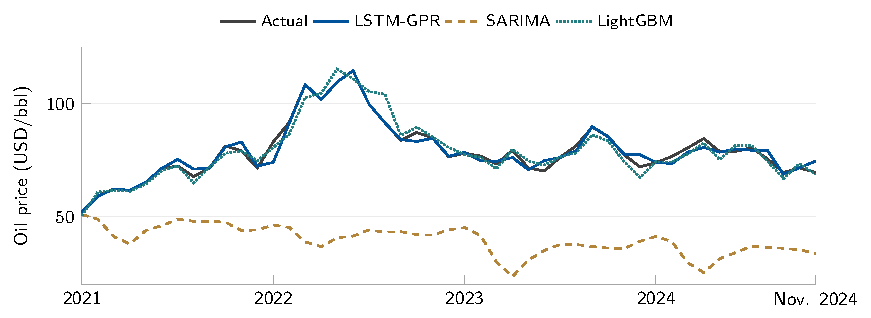
\includegraphics[width=37cm]{oil_comparison.pdf}};
\node[anchor=north west,inner sep=0,text width=37cm] at (3,85.0) {\captionfont LSTM-GPR: $R^2=0.963$, MAPE 1.86\%, RMSE 2.416 USD/bbl. Metrics were recomputed from 47 saved monthly comparison outputs; this is separate from the fixed-origin baseline exercise.};

\node[anchor=north west,inner sep=0,text width=37cm] at (3,90.5) {\posthead{04}{Open science and contact}};
\node[anchor=north west,inner sep=0] at (3.5,94.0) {\qrcode[height=5.3cm]{https://github.com/GreenComp-ERC/ImpactOfFossilFeulPrice}};
\node[anchor=north west,inner sep=0] at (13.0,94.0) {\qrcode[height=5.3cm]{https://huggingface.co/datasets/global-nomad-nexus/ImpactOfFossilFuelPrice-WACC}};
\node[anchor=north west,inner sep=0,text width=8cm,align=center,font=\fontsize{19}{24}\selectfont] at (2.15,99.9) {\textbf{Code + materials}};
\node[anchor=north west,inner sep=0,text width=8cm,align=center,font=\fontsize{19}{24}\selectfont] at (11.65,99.9) {\textbf{Dataset snapshot}};
\node[anchor=north west,inner sep=0,text width=15.7cm] at (22.5,94.0) {\fontsize{24}{31}\selectfont\textbf{\PresenterName}\\[0.2cm]\fontsize{19}{26}\selectfont\href{mailto:shilin.ou@dukekunshan.edu.cn}{\PresenterEmail}\\[0.35cm]\captionfont Editable LaTeX sources and corrected diagnostics are in the GitHub repository.};

% RIGHT COLUMN
\node[anchor=north west,inner sep=0,text width=37cm] at (44.1,29.5) {\posthead{05}{Regional model fit}};
\node[anchor=north west,inner sep=0] at (44.1,33.0) {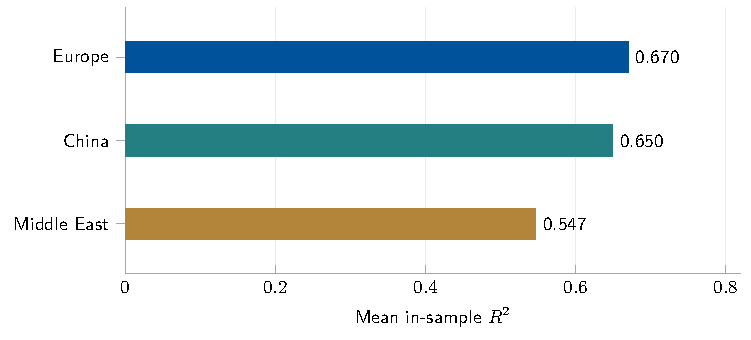
\includegraphics[width=37cm]{region_fit.pdf}};
\node[anchor=north west,inner sep=0,text width=37cm] at (44.1,51.3) {\captionfont Europe and China have stronger original in-sample fit. These $R^2$ values describe the joint fuel-price and inflation regressions; they do not measure price-shock magnitude.};

\node[anchor=north west,inner sep=0,text width=37cm] at (44.1,57.0) {\posthead{06}{Technology differences}};
\node[anchor=north west,inner sep=0] at (44.1,60.3) {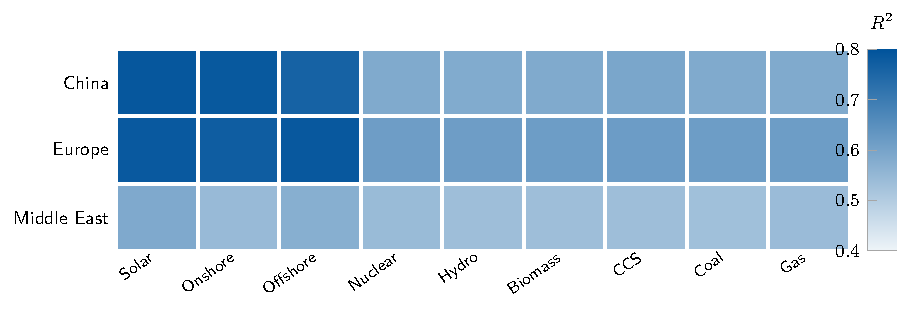
\includegraphics[width=37cm]{technology_fit.pdf}};
\node[anchor=north west,inner sep=0,text width=37cm] at (44.1,73.5) {\captionfont Mean $R^2$: solar 0.718; offshore wind 0.706; onshore wind 0.700. Other technologies average around 0.58. Cells average across fuels.};

\node[anchor=north west,inner sep=0,text width=37cm] at (44.1,77.5) {\posthead{07}{Chronological checks}};
\node[anchor=north west,inner sep=0] at (45.7,80.7) {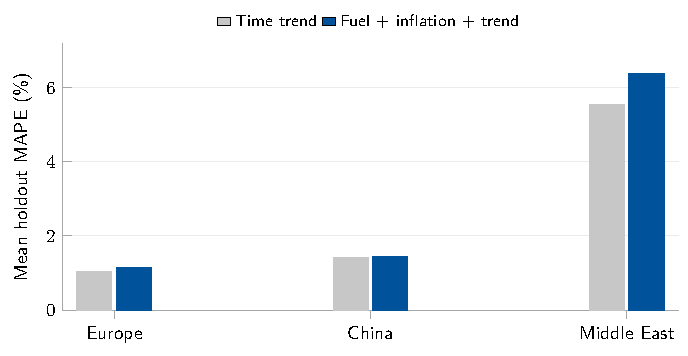
\includegraphics[width=33.0cm]{holdout_comparison.pdf}};
\node[anchor=north west,inner sep=0,text width=37cm] at (44.1,99.3) {\captionfont Ridge holdout, 2033--2035. Fuel + inflation + trend improves out-of-sample $R^2$ over a time trend in China 8/27, Europe 6/27, and Middle East 6/27 cases.};

% CONSISTENT CREDITS AND REFERENCES
\draw[Teal,line width=1.7pt] (3,104.2)--(81.1,104.2);
\node[anchor=north west,inner sep=0,text width=37cm] at (3,105.0) {\footfont
\textbf{\textsuperscript{*}Correspondence and affiliation}\par
\CorrespondenceText\par\vspace{0.4cm}
\textbf{Selected references}\par
Ameli et al., \textit{Nature Communications} 12, 4046 (2021). doi:10.1038/s41467-021-24305-3.\par
Calcaterra et al., \textit{Nature Energy} 9, 1241--1251 (2024). doi:10.1038/s41560-024-01606-7.\par
Paranhos, \textit{International Journal of Forecasting}, online 2025. doi:10.1016/j.ijforecast.2024.07.010.
};
\node[anchor=north west,inner sep=0,text width=37cm] at (44.1,105.0) {\footfont
\textbf{Acknowledgments}\par
\FundingText\par\vspace{0.25cm}
\textsuperscript{\dag}\AuthorNoteText\par\vspace{0.25cm}
\PreparationText
};
\end{scope}
\end{tikzpicture}
\end{document}
